\section*{Introduction}
Dans ce chapitre, nous présenterons le jeu de données. Des analyses MIDI-Audio
seront effectuées sur ce jeu de données par le biais de comparaisons de
transcription et transcriptions manuelles avec lilypond. Nous aborderons aussi,
le passage du monophonique au polyphonique, indispensable pour l’application
des formes rythmiques dans la chaîne de traitement. Nous présenterons une
réécriture guidée par une forme rythmique qui devra être utilisé comme base de
connaissances pour augmenter la rapidité et la qualité en sortie de qparse et
comme une méthode de création de nouvelles formes rythmiques. Enfin, nous
discuterons sur l’ensemble des travaux finis, notamment les avancées réalisées
dans ce travail.

\section{Le jeu de données}
\label{gmd}
Nous avons utilisé le Groove MIDI
Dataset\footnote{\url{https://magenta.tensorflow.org/datasets/groove}}
\cite{groove2019} (GMD) qui est un jeu de données mis à disposition par Google
sous la licence Creative Commons Attribution 4.0 International (CC BY 4.0).\\
Le GMD est composé de 13,6 heures de batterie sous forme de fichiers MIDI et
audio alignés. Il contient 1150 fichiers MIDI et plus de 22 000 mesures de
batterie dans les styles les plus courants et avec différentes qualités de jeu.
Tout le contenu a été joué par des humains sur la batterie électronique Roland
TD-11 (figure \ref{electro_drums}).
\begin{figure}[h]
	\centering
	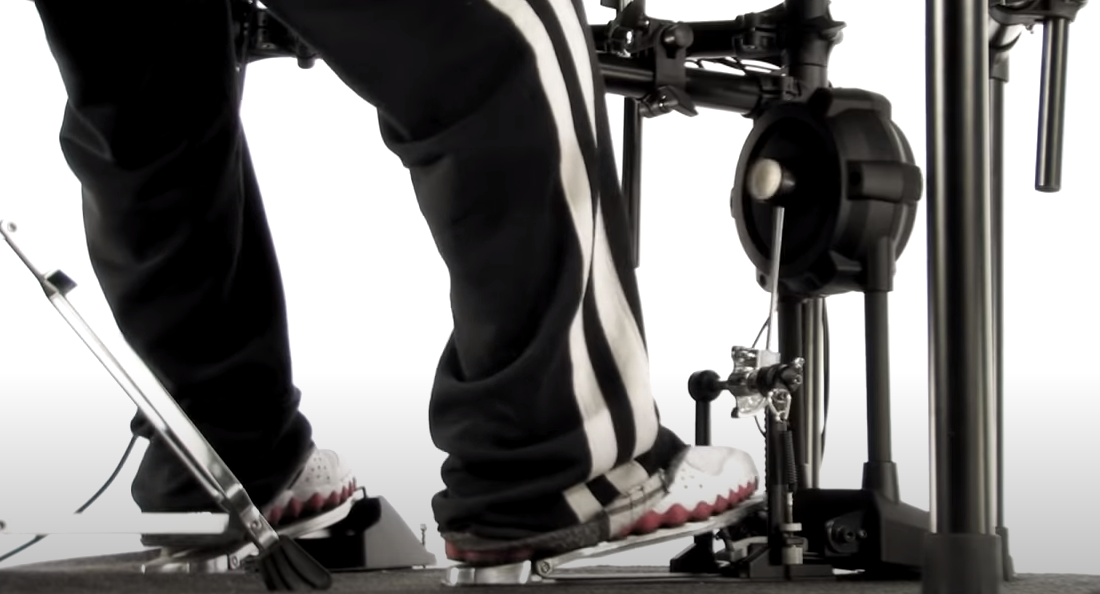
\includegraphics[height=35mm, width=60mm]
    {z_images/4_experimentations/0_groove/0_roland.png}\ \ 
	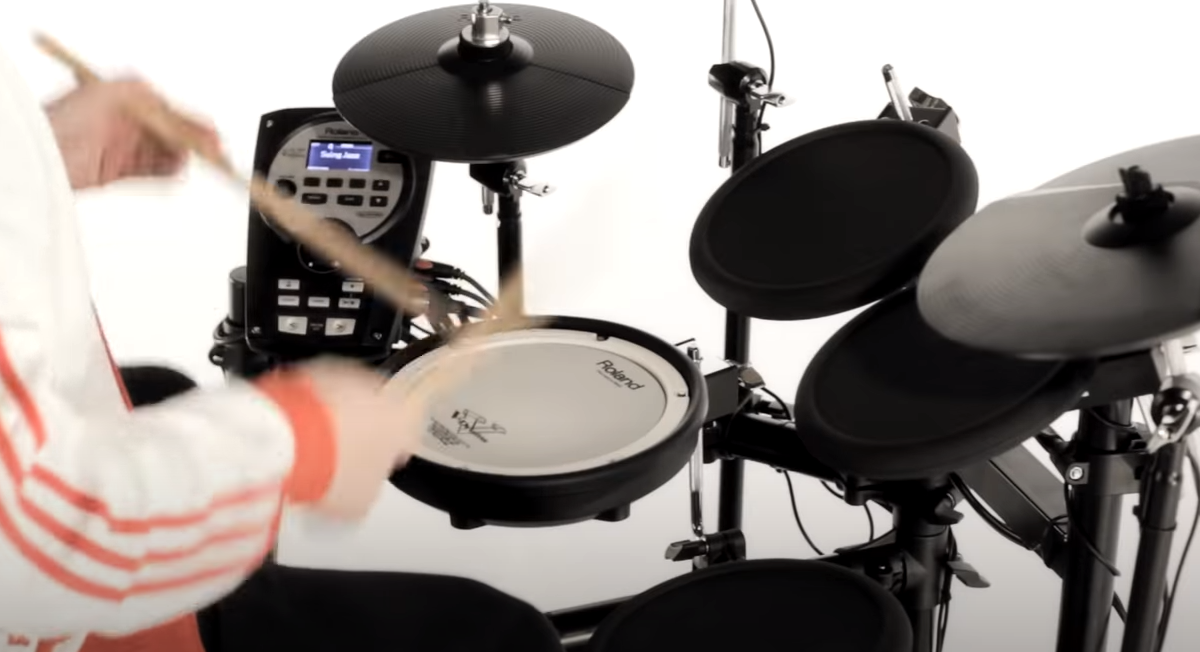
\includegraphics[height=35mm, width=60mm]
    {z_images/4_experimentations/0_groove/1_roland.png}
	\caption[Batterie électronique Roland TD-11]{Batterie électronique Roland
TD-11\footnotemark}
	\label{electro_drums}
	
\end{figure}
\footnotetext{\textit{Source~ :} \url{
    https://www.youtube.com/watch?v=BX1V_IE0g2c}}
Autres critères spécifiques au GMD~ :
\begin{itemize}
	\item Toutes les performances ont été jouées au métronome et à un tempo
        choisi par le batteur.
	\item 80\% de la durée du GMD a été joué par des batteurs professionnels
        qui ont pu improviser dans un large éventail de styles. Les données
        sont donc diversifiées en termes de styles et de qualités de jeu
        (professionnel ou amateur).
	\item Les batteurs avaient pour instruction de jouer des séquences de
        plusieurs minutes ainsi que des fills\footnote{Un \textit{fill} est une
        séquence de relance dont la durée dépasse rarement 2 mesures. Il est
        souvent joué à la fin d’un cycle pour annoncer le suivant.}.
	\item Chaque performance est annotée d’un style (fourni par le batteur),
        d’une signature rythmique et d’un tempo ainsi que d’une identification
        anonyme du batteur.
	\item Il a été demandé à 4 batteurs d’enregistrer le même groupe de 10
        rythmes dans leurs styles respectifs. Ils sont dans les dossiers
        eval-session du GMD.
	\item Les sorties audio synthétisées ont été alignées à 2 ms près sur leur
        fichier MIDI.
\end{itemize}

\subsection*{Format des données}
Le Roland TD-11 enregistre les données dans des fichiers MIDI et les divise en
plusieurs pistes distinctes~ :
\begin{itemize}
	\item une pour le tempo et l’indication de mesure~ ;
	\item une pour les changements de contrôle (position de la pédale de
        charley)~ ;
	\item une pour les notes.\\
\end{itemize}
Les changements de contrôle sont placés sur le canal 0 et les notes sur le
canal 9 (qui est le canal canonique pour la batterie).\\
Pour simplifier le traitement de ces données, ces trois pistes ont été
fusionnées en une seule piste qui a été mise sur le canal 9.

\section{Analyses et transcriptions manuelles}
\label{analyses_et_TM}
Ces analyses ont été faites dans le cadre de transcriptions manuelles à partir
de fichiers MIDI et Audio du GMD.

\subsection*{Comparaisons de transcriptions}
Pour les comparaisons de transcriptions, les transcriptions manuelles (TM) ont
été éditées à l’aide de Lilypond\footnote{\url{http://lilypond.org/}} ou
MuseScore\footnote{\url{https://musescore.com/}} et les transcriptions
automatiques (TA) ont toutes été générées par import d’un fichier MIDI dans
MuseScore.

\subsubsection{Exemple d’analyse 1}
\begin{figure}[h]
\centering
Transcription manuelle $\Rightarrow$ Transcription automatique
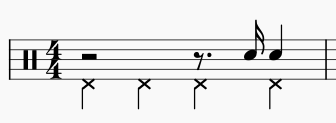
\includegraphics[height=20mm, width=50mm]{
z_images/4_experimentations/1_analyses/0_drummer1_session3/1_manuelle.png}
\ \ \ \ 
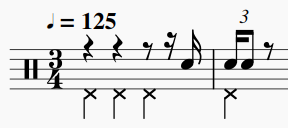
\includegraphics[height=20mm, width=45mm]{
z_images/4_experimentations/1_analyses/0_drummer1_session3/0_musescore.png}
\end{figure}
\begin{itemize}
	\item Erreur d’indication de mesure (3/4 au lieu de 4/4)~ ;
	\item Les silences de la mesure 1 de la TA sont inutilement surchargés~ ;
	\item La noire du temps 4 de la mesure 1 de la TM est devenue les deux
        premières notes (une double-croche et une croche) d’un triolet sur le
        temps 1 de la mesure 2 de la TA.
\end{itemize}

\subsubsection{Exemple d’analyse 2}
\begin{figure}[h]
\centering
\tab Transcription manuelle $\Rightarrow$ Transcription automatique\\
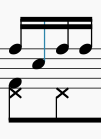
\includegraphics[height=20mm, width=13mm]{
z_images/4_experimentations/1_analyses/0_drummer1_session3/5_manuelle.png}
\ \ \ \ 
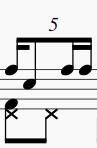
\includegraphics[height=20mm, width=13mm]{
z_images/4_experimentations/1_analyses/0_drummer1_session3/4_musescore.png}
\end{figure}
\begin{itemize}
	\item Les doubles croches ont été interprétées en quintolet
	\item La deuxième double-croche est devenue une croche.
\end{itemize}

\subsubsection{Exemple d’analyse 3}
\begin{figure}[h]
\centering
Transcription manuelle $\Rightarrow$ Transcription automatique
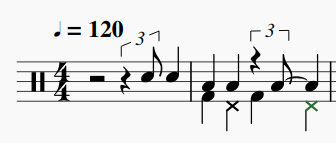
\includegraphics[height=24mm, width=50mm]{
z_images/4_experimentations/1_analyses/0_drummer1_session3/3_manuelle.png}
\ \ \ \ 
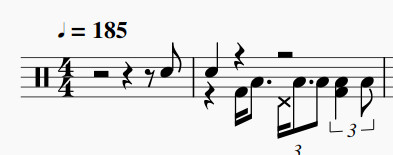
\includegraphics[height=25mm, width=55mm]{
z_images/4_experimentations/1_analyses/0_drummer1_session3/2_musescore.png}
\end{figure}

\begin{itemize}
	\item Les grosses-caisses, les charleys et les caisses-claires ont été
        décalés d’un temps vers la droite.
	\item Les toms basses des temps 1 et 2 de la mesure 2 de la TM ont été
        décalés d’une double croche vers la droite dans la TA.
	\item La première caisse claire de la mesure 1 devient binaire dans la TA
        alors qu’elle appartenait à un triolet dans la TM.
	\item Le triolet de tom-basse du temps 4 de la mesure 2 de la TA n’existe
        pas la TM.\\
\end{itemize}

\subsubsection{Exemple d’analyse 4}
\tab \tab Transcription manuelle $\Rightarrow$ Transcription automatique
\begin{figure}[h]
\centering
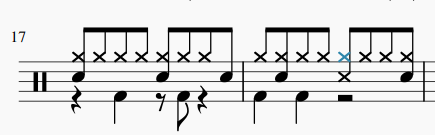
\includegraphics[height=19mm, width=50mm]{
z_images/4_experimentations/1_analyses/1_drummer1_session1/3_manuelle.png}
\ \ \ \ 
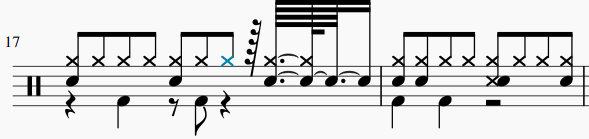
\includegraphics[height=19mm, width=70mm]{
z_images/4_experimentations/1_analyses/1_drummer1_session1/2_musescore.png}
\end{figure}

Sur le temps 4 de la mesure 1, la deuxième croche a été transcrite d’une
manière excessivement complexe!

\subsubsection{Exemple d’analyse 5 (flas)}
\label{flas}
Transcription manuelle\\
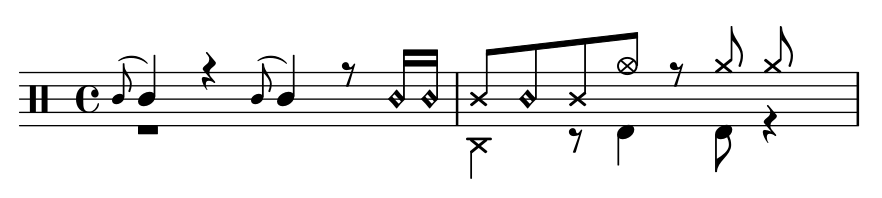
\includegraphics[height=25mm, width=95mm]{
z_images/4_experimentations/1_analyses/2_flas/0_124_funk_95_fill_4-4.png}\\
Transcription automatique\\\\
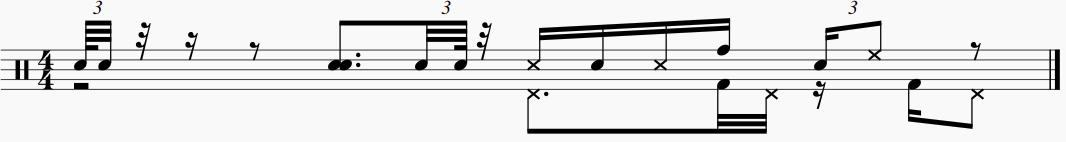
\includegraphics[height=20mm, width=130mm]{
z_images/4_experimentations/1_analyses/2_flas/1_124_funk_95_fill_4-4.png}\\

\begin{itemize}
	\item Le premier fla est reconnu comme étant un triolet contenant une
        quadruple croche suivie d’une triple croche au lieu d’une seule note
        ornementée.
	\item Le deuxième fla est reconnu comme étant un accord.
	\item Les deux double en contre-temps sur le temps 4 de la TM sont mal
        quantifiée dans la TA. 
	\item La TA ne reconnaît qu’une mesure quand la TM en transcrit deux. En
        effet, la TA a divisé par deux la durée des notes afin de les faire
        tenir dans une mesure à 4 temps dont les unités de temps sont les
        noires. Par exemple, le soupir du temps 2 de la TM devient un
        demi-soupir sur le contre-temps du temps 1 dans la TA. Ou encore, la
        noire (pf, voir le tableau \ref{pitchs_instru}) sur le temps 1 de la
        mesure 2 de la TM suivie d’un demi-soupir devient une croche pointée
        sur le temps 3 de la TA.
	\item Autre problème~ : certaines têtes de notes sont mal attribuées. Par
        exemple, le charley ouvert en contre-temps sur le temps 2 de la mesure
        2 de la TM devrait avoir le même symbole sur la TA. Idem pour les
        cross-sticks.
\end{itemize}

\subsubsection{Conclusion d’analyse}
Ces analyses ont montré la difficulté pour un logiciel comme MuseScore d’offrir
une partition lisible. Les raisons sont le fait que les fichiers MIDI ne sont
pas encore quantifiés mais aussi qu’il n’y a pas de reconnaissance de la forme 
du rythme impliquant sa position dans la mesure. Cette reconnaissance pourrait
permettre de rectifier les problèmes de signature rythmique ainsi que les
problèmes de décalage de temps. La reconnaissance de la forme du rythme
permettrait aussi de supprimer les aberrations du type de celle de l’exemple
d’analyse 4, puisque l’erreur sur cet exemple serait reconnue comme un élément
qui ne rentre pas dans le cadre de la forme de rythme en question. La dernière
raison qui rend le travail difficile est l’identification des flas, comment
savoir si deux notes jouées très proches sont~ :
\begin{itemize}
    \item séparées et rapides,
    \item mal jouées à l’unisson (accord),
    \item ou forment un fla ?
\end{itemize}


\subsection*{Transcription de partition}
\label{partition_entiere}
La figure \ref{partition_ref} est la transcription manuelle des fichiers
\textit{004\_jazz-funk\_116\_beat\_4-4.mid} et
\textit{004\_jazz-funk\_116\_beat\_4-4.wav} du GMD.

Cette transcription a été entièrement faite avec Lilypond (voir le code
lilypond sur le git \url{https://github.com/MartinDigard/Stage_M2_Inria}). Il
s’agit d’une partition d’un 4/4 binaire dont le fichier MIDI est annoncé dans
le GMD de style «~jazz-funk~» probablement en raison de la ride de type shabada
rapide (le ternaire devient binaire avec la vitesse) combiné avec l’after-beat
de type rock (caisse claire sur les deux et quatre).

La transcription manuelle de la partition de la figure \ref{partition_ref} et
l’analyse d’autre fichiers MIDI (voir section \ref{analyses_et_TM}) m’ont mené
aux observations suivantes~ :
\begin{itemize}
	\item Vélocité inférieure à 40~ : ghost-note.
	\item Vélocité supérieure à 90~ : accent.
	\item Pas d’intention d’accent ni de ghost-note pour une vélocité entre 40
        et 89.
	\item Les accents et les ghosts-notes ne sont significatifs ni pour les
        instruments joués au pied, ni pour les cymbales crash.\\
	En effet, certaines vélocités en dessous de 40 étant détectées et inscrites
    dans les données MIDI sont dues au mouvement du talon du batteur qui bat la
    pulsation sans particulièrement jouer le charley. Ce mouvement est perçu
    par le capteur de la batterie électronique mais le charley n’est pas joué.
	\item Au final, j’ai relevé les ghost-notes et les accents pour la caisse
        claire ainsi que les accents pour les toms et les cymbales rythmiques
        (charley et ride).
\end{itemize}


\subsubsection{Conclusion sur les transcriptions manuelles}
La transcription des données audio et MIDI contenues dans ces fichiers a permis
une analyse plus approndie des critères à relever pour chaque évènement MIDI et
de la manière de les considérer dans un objectif de transcription en partition
lisible pour un musicien (Voir la section \ref{modelisation_transcription}).


\section{Transcription polyphonique par \textit{parsing}}
\label{jam}
Les Jams permettent de passer du monophonique au polyphonique.
On regroupe tous les évènements qu’on estime être à des dates suffisamment
proches dans des clusters que nous avons appelés «~Jam~».
Un Jam représente une séquence de points successifs dans un segment d’entrée
avec des informations supplémentaires sur leur rôle respectif, en supposant
qu’ils sont tous alignés à la même date lors de la quantification. Un Jam est
caractérisé par l’index de son premier point dans le segment d’entrée et sa
longueur (nombre de points).
Une fois dans les Jams, les évènements sont identifiés selon les critères
suivants~ :
\begin{itemize}
    \item \textit{Ignored}, les offsets sont ignorés~ ;
    \item \textit{Note}, si c’est une note simple~ ;
    \item \textit{Rest}, si c’est un silence~ ;
    \item \textit{GraceNote}, si c’est un fla~ ;
    \item \textit{Error}.
\end{itemize}

\section{Réécriture guidée par une forme rythmique}
\label{reecriture_guidee}
La démonstration qui suit est basée sur la partition de référence de la figure
\ref{partition_ref} puisque la forme rythmique qui sera utilisée en est
directement extraite.\\

Nous allons montrer~ :
\begin{itemize}
    \item la composition de cette forme rythmique~ ;
    \item son état final, c’est à dire toutes les combinaisons entièrement
        écrites en notation correcte sur partition~ ;

        $\Rightarrow$ cela constituera une référence pour la réécriture~ ;
    \item un exemple de transformation de la forme rythmique en arbre de
        rythme~ ;
    \item l’application de la séparation des voix sur cet exemple basé sur la
        référence citée précédemment (la forme rythmique en question)~ ;\\
        $\Rightarrow$ l’arbre de départ sera alors séparé en autant d’arbres
        qu’il y a de voix (deux arbres pour cette forme rythmique)~ ;
    \item les règles de simplification propres à la forme rythmique dont nous
        parlons. 
\end{itemize}
L’objectif de cette démonstration est de montrer comment un jeu de plusieurs
formes rythmiques pourrait être implémenté dans le cadre d’une approche
dictionnaire.

\subsection*{Motifs et gammes}
\begin{figure}[h]
\centering
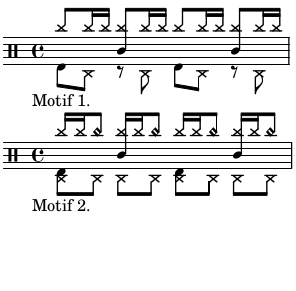
\includegraphics[height=43mm, width=40mm]{
z_images/4_experimentations/2_reecriture_guidee/0_motifs_4-4_binaires.png}
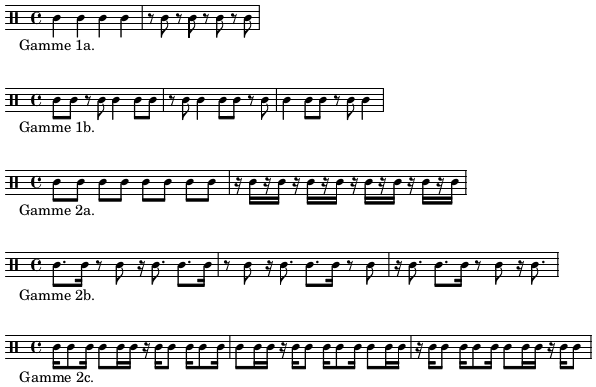
\includegraphics[height=55mm, width=85mm]{
z_images/4_experimentations/2_reecriture_guidee/1_gammes_4-4_binaires.png}
\caption{Motifs et gammes}
\label{motifs_gammes}
\end{figure}

\subsubsection{Motifs}
À partir de la partition de référence, les deux motifs de la figure
\ref{motifs_gammes} peuvent être systématisés. Le motif 1 est joué du début
jusqu’à la mesure 18 avec des variations et des fills et le motif 2 est joué de
la mesures 23 à la mesure 28 avec des variations. Ces deux motifs sont très
classiques et pourront être détectés dans de nombreuses performances.\\

\subsubsection{Gammes}
Les gammes de la figure \ref{motifs_gammes} étayent toutes les combinaisons
d’un motif en 4/4 binaires jusqu’aux doubles croches.\\
Les lignes 1 et 2 traitent les croches. La ligne 1 a 2 mesures dont la première
ne contient que des noires et la deuxième que des croches en contre-temps. Ces
deux possibilités sont combinées de manière circulaire dans les 3 mesures de la
deuxième ligne.\\
Les lignes 3, 4 et 5 traitent les doubles-croches. La ligne 3 a 2 mesures dont
la première ne contient que des croches et la deuxième que des doubles-croches
en contre-temps. Ces deux possibilités sont combinées de manière circulaire
dans les lignes 4 et 5 qui contiennent chacunes 3 mesures.

\subsection*{Formes rythmiques — motifs et gammes combinés}
Pour la suite de cette démonstration, j’utiliserai le motif 1 de la
figure \ref{motifs_gammes}.
\begin{figure}[h]
\centering
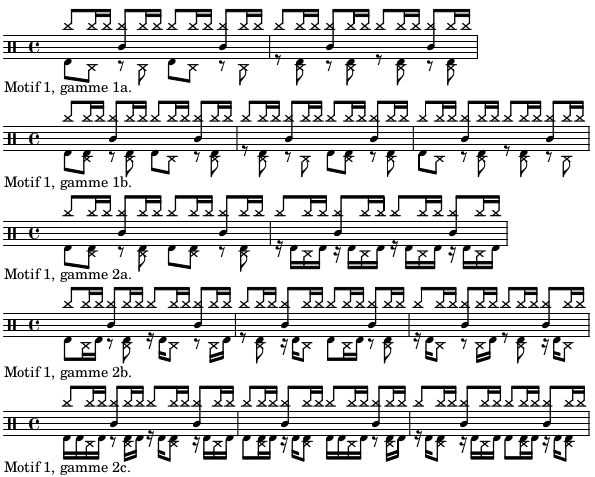
\includegraphics[height=75mm, width=85mm]{
z_images/4_experimentations/2_reecriture_guidee/2_systeme_4-4_binaire.png}
\caption{Partition d’un forme rythmique en 4/4 binaire}
\label{sys_binaire}
\end{figure}
\subsection*{Représentation de la forme rythmique en arbres de rythmes}
\label{demo_sys}
\begin{figure}[h]
	\centering
	\resizebox{350pt}{!} {
		\Tree[.Motif\ 1\ +\ gamme\ 1a
		[.Mesure\ 1
		[.Temps\ 1 [rd\\bd ][ [rd\\pf ][rd ]]]
		[.Temps\ 2 [rd\\cc ][ [rd\\pf ][rd ]]]
		[.Temps\ 3 [rd\\bd ][ [rd\\pf ][rd ]]]
		[.Temps\ 4 [rd\\cc ][ [rd\\pf ][rd ]]] ]
		[.Mesure\ 2
		[.Temps\ 1 [rd ][ [rd\\bd\\pf ][rd ]]]
		[.Temps\ 2 [rd\\cc ][ [rd\\bd\\pf ][rd ]]]
		[.Temps\ 3 [rd ][ [rd\\bd\\pf ][rd ]]]
		[.Temps\ 4 [rd\\cc ][ [rd\\bd\\pf ][rd ]]] ]]}
	\caption{Représentation arborescente d’une forme rythmique}
	\label{arbre_sys}
\end{figure}
L’arbre de la figure \ref{arbre_sys} servira de base pour le suite de
l’expérimentation. Comme indiqué à la racine de l’arbre, il représente la
première ligne de la figure \ref{sys_binaire}. Même si cet arbre représente
parfaitement le rythme concerné, il manque des indications de notation telles
que les voix spécifiques à chaque partie du rythme ainsi que les choix
d’écriture pour les distances qui séparent les notes de chaque voix entre elles
en termes de durée.

\subsection*{Réécriture — séparation des voix et simplification}
\subsubsection{La séparation des voix}
Ainsi l’arbre syntaxique de départ est divisé en autant d’instruments qui le
constituent et les voix sont regroupées en suivant les régles de la forme
rythmique.
\begin{figure}[h]
	\centering
	\resizebox{350pt}{!} {
		\Tree[.Motif\ 1\ +\ Gamme\ 1a
		[.Mesure\ 1
		[.Temps\ 1 [rd ][ [rd ][rd ]]]
		[.Temps\ 2 [rd\\cc ][ [rd ][rd ]]]
		[.Temps\ 3 [rd ][ [rd ][rd ]]]
		[.Temps\ 4 [rd\\cc ][ [rd ][rd ]]] ]
		[.Mesure\ 2
		[.Temps\ 1 [rd ][ [rd ][rd ]]]
		[.Temps\ 2 [rd\\cc ][ [rd ][rd ]]]
		[.Temps\ 3 [rd ][ [rd ][rd ]]]
		[.Temps\ 4 [rd\\cc ][ [rd ][rd ]]] ]]}
	\caption{arbre de rythmes — voix haute}
	\label{voix_haute}
\end{figure}\\
La voix haute (figure \ref{voix_haute}) regroupe la ride et la caisse claire
sur les ligatures du haut.
\begin{figure}[h]
	\centering
	\resizebox{350pt}{!} {
		\Tree[.Motif\ 1\ +\ Gamme\ 1a
		[.Mesure\ 1
		[.Temps\ 1 [bd ][ [pf ][t ]]]
		[.Temps\ 2 [t ][ [pf ][t ]]]
		[.Temps\ 3 [bd ][ [pf ][t ]]]
		[.Temps\ 4 [t ][ [pf ][t ]]] ]
		[.Mesure\ 2
		[.Temps\ 1 [t ][ [bd\\pf ][t ]]]
		[.Temps\ 2 [t ][ [bd\\pf ][t ]]]
		[.Temps\ 3 [t ][ [bd\\pf ][t ]]]
		[.Temps\ 4 [t ][ [bd\\pf ][t ]]] ]]}
	\caption{arbre de rythmes — voix basse}
	\label{voix_basse}
\end{figure}\\
La voix basse (figure \ref{voix_basse} regroupe la grosse caisse et le charley
au pied sur les ligatures du bas.
\subsubsection{Les règles de simplifications}
L’objectif des règles de simplifications est de réécrire les écarts de durée
qui séparent les notes d’une manière appropriée pour la batterie et qui soit la
plus simple possible. Les ligatures relient les notes d’un temps entre elles
afin de rendre la pulsation visuelle.\\\\
Pour les figures ci-dessous~ :
\begin{itemize}
	\item x = une note~ ;
	\item r = un silence~ ;
	\item t = une continuation (point ou liaison)
\end{itemize}
\begin{figure}[h]
	\centering
	\resizebox{50pt}{!} {
		\Tree[.1/4 [x ][ [x ][t ]] ]
	}\ \ \ \ \ $\Rightarrow$\ \ \ \ \
	\resizebox{30pt}{!} {
		\Tree[.1/4 [x ][x ] ]
	}\\
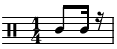
\includegraphics[height=10mm, width=25mm]{
z_images/4_experimentations/2_reecriture_guidee/simplification_0.png}\ \ \ \ \ 
$\Rightarrow$\ \ \ \ \
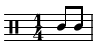
\includegraphics[height=10mm, width=20mm]{
z_images/4_experimentations/2_reecriture_guidee/simplification_1.png}
	\caption{Exemple de simplification 1}
	\label{1}
\end{figure}
\begin{figure}[h]
	\centering
	\resizebox{50pt}{!} {
		\Tree[.1/4 [t ][ [x ][t ]] ]
	}\ \ \ \ \ $\Rightarrow$\ \ \ \ \
	\resizebox{30pt}{!} {
		\Tree[.1/4 [r ][x ] ]
	}\\
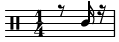
\includegraphics[height=10mm, width=25mm]{
z_images/4_experimentations/2_reecriture_guidee/simplification_2.png}\ \ \ \ \ 
$\Rightarrow$\ \ \ \ \
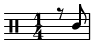
\includegraphics[height=10mm, width=20mm]{
z_images/4_experimentations/2_reecriture_guidee/simplification_3.png}
	\caption{Exemple de simplification 2}
	\label{2}
\end{figure}
\begin{figure}[h]
	\centering
	\resizebox{70pt}{!} {
		\Tree[.1/4 [x ][t ][x ][x ]]
	}\ \ \ \ \ $\Rightarrow$\ \ \ \ \
	\resizebox{50pt}{!} {
		\Tree[.1/4 [x ][ [x ][x ]]]
	}\\
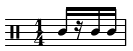
\includegraphics[height=10mm, width=25mm]{
z_images/4_experimentations/2_reecriture_guidee/simplification_4.png}\ \ \ \ \ 
$\Rightarrow$\ \ \ \ \
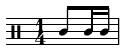
\includegraphics[height=10mm, width=20mm]{
z_images/4_experimentations/2_reecriture_guidee/simplification_5.png}
	\caption{Exemple de simplification 3}
	\label{3}
\end{figure}\newpage
\begin{figure}[h]
	\centering
	\resizebox{70pt}{!} {
		\Tree[.1/4 [t ][x ][x ][t ] ]
	}\ \ \ \ \ $\Rightarrow$\ \ \ \ \
	\resizebox{50pt}{!} {
		\Tree[.1/4 [ [r ][x ]][x ] ]
	}\\
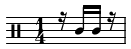
\includegraphics[height=10mm, width=25mm]{
z_images/4_experimentations/2_reecriture_guidee/simplification_8.png}\ \ \ \ \ 
$\Rightarrow$\ \ \ \ \
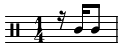
\includegraphics[height=10mm, width=25mm]{
z_images/4_experimentations/2_reecriture_guidee/simplification_9.png}
	\caption{Exemple de simplification 4}
	\label{4}
\end{figure}
%\newpage
Ces règles ont été tirées de l’ensemble des arbres de la forme rythmique.

Les règles remplacent par un silence les continuations (t) qui sont au début
d’un temps. Cela est valable pour cette forme rythmique mais lorsqu’il y a des
ouvertures de charley, cela n’est pas toujours applicable.

\subsection*{Conclusion sur cette réécriture guidée}
La méthode des formes rythmiques étant basée sur une approche dictionnaire,
le premier objectif de cette réécriture guidée est d’orienter la recherche
d’autres formes rythmiques par observation du jeu de données et de montrer
comment les construire pour agrandir la base de connaissance de qparse pour la
transcription de la batterie.

\section{Discussion}

TRAVAUX EFFECTUÉS
\subsection*{Formes rythmiques, notation et modélisation de la batterie}
Un système de formes rythmiques imposant chacune ses régles propres pour
l’écriture de partitions de batterie a été formalisé. Une démonstration
théorique de ce système a permis de montrer comment créer des formes rythmiques
avec leurs régles propres
à partir de partitions de référence pour agrandir un dictionnaire de formes
rythmiques. La théorie pour l’application des formes rythmiques sur un arbres
de \textit{parsing} en \textit{input} de qparse pour appliquer les règles de réécriture
a été formalisé. Durant ce travail, la modélisation de la notation particulière
de la batterie a été effectuée, notamment sur toutes les particularités qui
concerne l’écriture des distances temporelles entre les notes.\\

Il y a deux dimensions de le travail fourni~ :
\begin{enumerate}
    \item la volonté de pousser un exemple simple jusqu’au bout de la chaîne
        pour obtenir des résultats et une évaluation sur au moins un exemple~ ;
    \item la réalité du travail à fournir pour faire avancer la chaîne de
        traitement car sans sortie possible en bout de chaîne, aucun test ne
        peut être effectué…
\end{enumerate}

Une solution aurait été de considérer les arbres de \textit{parsing} obtenus après le
traitement du polyphonique comme un résultat local possible à évaluer au lieu
d’attendre que la chaîne arrive jusqu’à la génération d’une partition mais cela
n’était pas prioritaire pendant le stage.

\subsection*{Scripts lilypond}
Le choix de travailler avec lilypond au lieu de musescore a été pertinent car
il m’a permis d’établir une modélisation de la batterie avec une notation
cohérente accompagnée d’un fichier de configuration lilypond inspiré de la
notation Agostini et de nombreux exemples de scripts lilypond recouvrant
plusieurs phénomènes de notation en batterie utiles dans des contextes binaires
ou ternaires.

\subsection*{Passage au polyphonique}
Nous avons améliorer le système de quantification de qparse pour la batterie,
notamment le passage à la polyphonie grâce aux Jams qui ont permis
l’identification des regroupements de notes. Dans ce cadre, j’ai formalisé des
régles pour la reconnaissance des flas et proposé un système de seuil basé sur
la distance entre deux notes proches (donc regroupées dans un Jam) et qui
permet de définir si les deux notes sont proches et quantifiables, si elles
forment un fla ou si elles forment simplement un accord.

Ce travail a permis d’obtenir, avec la création de grammaire adéquates, des
arbres de \textit{parsing} corrects en sortie de qparse avec des exemples simples de
fichiers MIDI en entrée.\\

TRAVAUX FUTURS
\subsection*{Agrandir le dictionnaire de formes rythmiques}
Les formes rythmiques, qui constituent la proposition de ce mémoire,
nécessitent encore beaucoup de travail pour pouvoir être évaluées. Comme il
s’agit d’une approche dictionnaire, il faudrait créer beaucoup de formes
différentes avec chacune leur propres règles. L’objectif étant que cette
approche dictionnaire laisse la place à une génération de formes rythmiques en
par apprentissage sur des données.

\subsection*{Finir la chaîne de traitement}
Pour qu’une réelle évaluation soit possible, il faut que la chaîne de
traitement aille jusqu’à la génération d’une partition finale (après séparation
des voix et règles de réécriture). Expérimenter les motifs sur plusieurs
exemples aurait été indispensable pour obtenir une quantité de résultats qui
justifieraient une évaluation automatique permettant de faire des graphiques afin
d’éprouver efficacement le système des formes rythmiques. Il faudrait donc
élaborer plus d’exemples de grammaires qui puissent fonctionner avec des
signatures rythmiques différentes.\\

\subsection*{lilypond pour l’évaluation}
Le fait que lilypond utilise du texte (scripts) pour générer des partitions en
pdf pourrait permettre d’élaborer un système d’évaluation en utilisant la
comparaison de données textuelles. On pourrait par exemple, configurer
l’\textit{ouput} de qparse au format lilypond pour ensuite comparer une
partition de référence transcrite manuellement avec lilypond sur la sortie.
Comme il s’agit de comparer deux scripts, cette comparaison pourrait être
effectuée avec la commande «~diff~» .
